\documentclass[10pt]{article}

%%%%%%%%%Includes%%%%%%%%%%%%%%%%%%%%%%%%%%%%%
\usepackage[a4paper, total={7.5in, 11in}]{geometry}
\usepackage{amsmath}
\usepackage{amsfonts}
\usepackage{graphicx}
\usepackage{hyperref}
\pagenumbering{gobble}


%%%%%%%%%tikz%%%%%%%%%%%%%%%%%%%%%%%%%%%%%%%%%%%%%%%%%%%%


\title{Stroke Prediction with Decision Trees}
\date{\today}
\author{Thomas Bourton}

\begin{document}
\maketitle 
\section{Problem Description}
Predictive model: We use a predictive model to classify patients who have
stroke. We evaluate the performance of the model and suggest which features may be
useful in stroke prediction.

Based on the \texttt{​train\_2v.csv} from the Kaggle stroke dataset: \href{https://www.kaggle.com/asaumya/healthcare-dataset-stroke-data}{www.kaggle.com/asaumya/healthcare-dataset-stroke-data}
​

\section{Preliminary Analysis and Visualisation}
The training data contains data regarding stroke patients. The feature variables are \texttt{gender, age, hypertension, heart\_disease, ever\_married, work\_type, residence\_type, avg\_glucose\_level, bmi, smoking\_status} while the target variable is \texttt{stroke}. The training dataset contains 43400 entries of which approximately 1.8\% have stroke. 

Our aim is to determine which features are most important in determining whether a given person has stroke or not. Hence it is useful to separate the data into those patients with stroke and those without. We can make some preliminary plots. For example, one might expect that e.g. a patient who has never suffered from heart disease is less likely to have stroke and vice versa. We can plot this (see Figure \ref{fig1}) and it somewhat confirms our initial estimate.
\begin{figure}[h!]
\centering  
\begin{minipage}[b]{0.45\textwidth}
    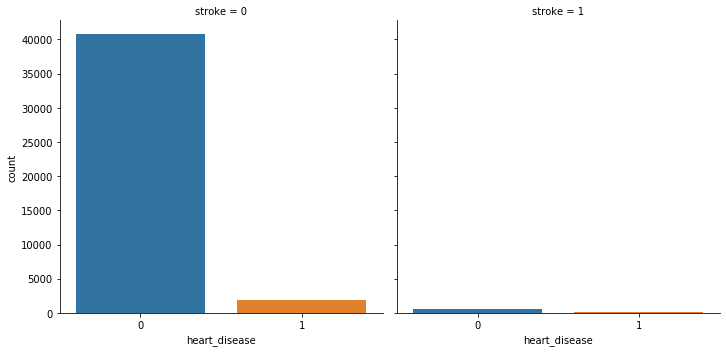
\includegraphics[width=\textwidth]{index.png}
  \end{minipage}
  \hfill
  \begin{minipage}[b]{0.45\textwidth}
    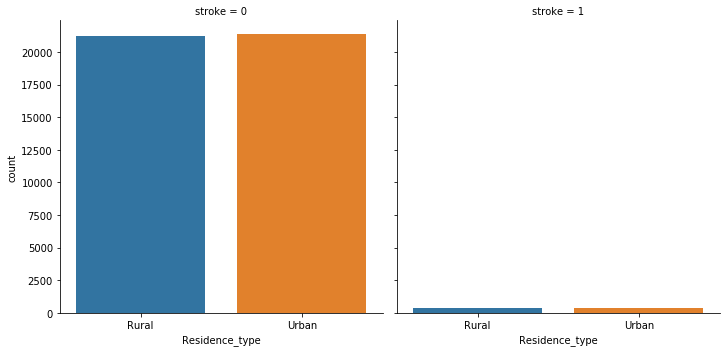
\includegraphics[width=\textwidth]{index2.png}
  \end{minipage}
\caption{Left: \textit{Number of patients with heart disease with/without stroke.} Right: \textit{Residence types having not with/without stroke.}}
\label{fig1}
\end{figure}
On the other hand, for example one would also expect that the area in which a patient lives (rural or urban) appears to have little direct importance in a medical condition such as stroke, see Figure \ref{fig1}. We can again plot this and be fairly confident that this initial assumption is somewhat correct.
We can also plot the age distribution for stroke/no-stroke. We can see that the proportion of patients with stroke is skewed heavily towards the ages 60+. There is similar patterns for average glucose level, a larger proportion of stroke patients have a high average glucose level. See Figure \ref{fig2}.
\begin{figure}[h!]
\centering  
\begin{minipage}[b]{0.45\textwidth}
    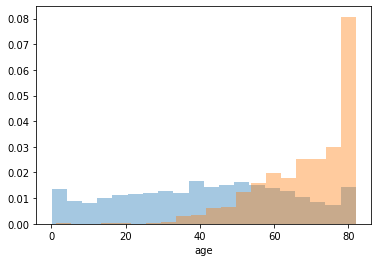
\includegraphics[width=\textwidth]{index3.png}
  \end{minipage}
  \hfill
  \begin{minipage}[b]{0.45\textwidth}
    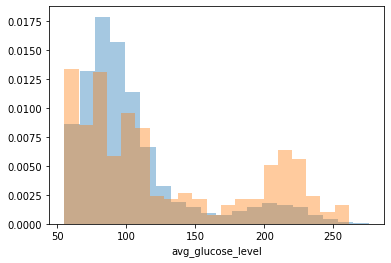
\includegraphics[width=\textwidth]{index1.png}
  \end{minipage}
\caption{Left: \textit{Distribution of ages without stroke (blue) / with stroke (orange).} Right: \textit{Average glucose level of patients without stroke (blue) / with stroke (orange).}}
\label{fig2}
\end{figure}
\section{Data Clean-up and Wrangling}
Having performed some basic analysis on our data we now would like to build our model. However before doing this we have to prepare the data. In particular we have two main concerns. The first is that both the training and test data have missing data for \texttt{bmi} and \texttt{smoking\_status}. Approximately 3\% of \texttt{bmi} data and 30\% of \texttt{smoking\_status} data is missing from both sets. For \texttt{bmi} data we will simply replace the missing data with the average for each set. On the other hand a much larger portion of \texttt{smoking\_status} data is missing, also this label is discrete hence replacing such a large proportion with an average is potentially troublesome. We will pursue two approaches, the first being to replace this data with the mode (which is never smoked) the second is to completely drop the \texttt{smoking\_status} data from the dataset.

The second main concern with the data contains is that it contains many categorical variables. The decision tree algorithm cannot deal with categorised data, hence we need to turn the features \texttt{ever\_married, work\_type, residence\_type, smoking\_status} into numerical variables. We do this using the dummy variables methods in the pandas library.
\section{Building Decision Tree Model}
We build the model with the \texttt{smoking\_status} data replaced by the mode. We then build the model using the feature variables with target being \texttt{stroke}. We are going to use the \texttt{tree} library from the \texttt{sklearn} package. In order to build the model we further split the training data into a trainset and a testset. We chose a $80/20$ split. We train the model on the trainset, this builds the predictive model. By using this model on the testset and comparing with the known data from the testset we can determine several analytical metrics on the model. The model with the smoking data replaced by mode performed with accuracy of 96.2\%.

We also repeated the same model build but with the smoking data removed. In which case the model was 96.1\% accurate at predicting stroke on the testset.
\section{Analysis of the Model and Conclusions}
Our main goal is to determine the importance of the features on determining stroke. Hence we can plot the feature importance metrics, see Figure \ref{fig3}. The models both confirm our early expectations that for example \texttt{age} and \texttt{bmi} are quite important in predicting stroke, whereas \texttt{residence\_type} is fairly unimportant. A surprising output of the model is that \texttt{heart\_disease} appears to be very unimportant in determining stroke, where the preliminary analysis suggested to expect otherwise.
\begin{figure}[h!]
\centering  
\begin{minipage}[b]{0.45\textwidth}
    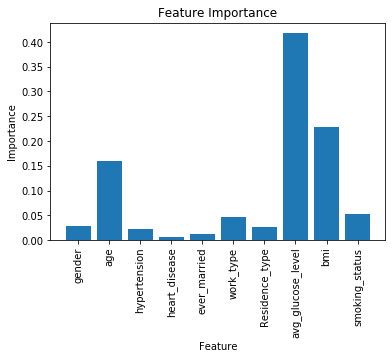
\includegraphics[width=\textwidth]{index4.png}
  \end{minipage}
  \hfill
  \begin{minipage}[b]{0.45\textwidth}
    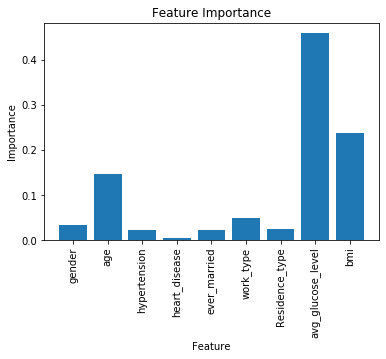
\includegraphics[width=\textwidth]{index5.png}
  \end{minipage}
\caption{Left: \textit{Feature importance for model with smoking data replaced by the mode.} Right: \textit{Feature importance with smoking data removed.}}
\label{fig3}
\end{figure}
We can also see that our model matches the approximate data visualisations in each case (see Jupyer notebook for more plots).
When applied to the test data with unknown stroke data the model with smoking replaced by the mode predicted that $350/18261\sim0.019$ fraction of patients have stroke, this is to be compared with $783/43400\sim0.018$ in the known training data.

One potential way that the model could be improved is by dealing more systematically with the smoking status data. Instead of simply replacing each missing entry with the mode we could have placed instead a more uniform distribution of data which could have been derived from the training data. This is important as one would naively think that smoking should have a larger impact on determining stroke than our model predicted.
\end{document}
